\dictum[F. Dostevski -- Crime and Punishment]{We may note in passing,
one peculiarity in regard to all the final resolutions taken by
[Raskolnikov] in the matter; they had one strange characteristic: the
more final they were, the more hideous and the more absurd they at
once became in his eyes. In spite of all his agonising inward
struggle, he never for a single instant all that time could believe in
the carrying out of his plans.}

\begin{summary}
\item We introduce a monad-based functional method of weighted
  backtracking search that supports \emph{once} and \emph{fallback},
  two cut-like operations.
\item The FluiDB query planner follows an \(A^{\star}\)-like method for
  searching plans are searched in a top-down fashion, guided by a
  cost model that takes into account the cost historical queries.
\item The query planner can make use of \emph{forward} or
  \emph{reverse} triggering of operators.
\item The garbage collector clears up space on demand maintaining the
  materializability of all n-nodes in the graph.
\end{summary}

This chapter goes in detail about the architecture of the logical
planing of a query. Query planning is based on an \(A^{\star}\)-like
search algorithm through the space of partial plans. We initially
describe the fundamental computational structures that facilitate this
search and their unique properties that allow us the necessary
flexibility. Then we discuss the basic backtracking algorithm and the
way the graph is traversed. We move on to discussing the garbage
collection that generates plan fragments that allow the plan to free
up space in the underlying storage. Finally, we talk about the cost
model that guides the plan search process.

\section{HCntT logic monad}

The FluiDB planner is designed in terms of a backtracking search
algorithm that searches in the space of subplans for an optimal
plan. Because the algorithm involves a lot of complicated heuristics
it is important that a powerful underlying framework is deployed that
matches the purely functional infrastructure in which FluiDB is
implemented.  In particular, we require a monad that supports both
weighted search and soft cuts. Because none of the solutions we found
in the literature support both we developed the \hask{HCntT}
backtracking monad that is described in this section.

\subsection{Background}

Monads for backtracking in a functional context have been proposed in
various incarnations.  The most common monad that encapsulates this functionality is the \hask{ListT} monad transformer
\hask{ListT m a = forall b . (a -> m b -> m b) -> m b -> m b}, also
dubbed the Church encoding of lists or an application of the Cayley
theorem on lists. It was first proposed (in an untyped form in
scheme) in \cite{haynesLogicContinuations1987} where Haynes explicitly
uses it to implement a logic programming framework back in 1987, but
most authors in the field cite
\cite{hinzeDerivingBacktrackingMonad2000a} as the seminal work on the
concept where the authors seem to have independently re-discovered the
application of the concept in 2000 this time in strongly typed ML, and also
\cite{kiselyovBacktrackingInterleavingTerminating} where the authors
focused on a notion of fairness in backtracking. As shown in
\cite{kidneyAlgebrasWeightedSearch2021} this representation has
\(O(n^2)\) BFS complexity.

The other common representation of a list monad transformer is the more
straightforward

\begin{haskellcode}
newtype ListT m a = ListT (Maybe (a,ListT m a))
\end{haskellcode}

Which mirrors precisely the idea behind \hask{MonadLogic} from
\cite{kiselyovBacktrackingInterleavingTerminating}. As demonstrated in
listing \ref{lst:monad_logic} the \hask{MonadLogic} able to
\hask{cons} (dubbed \hask{reflect} which directly corresponds to the \hask{ListT} constructor) and \hask{uncons} (dubbed
\hask{msplit} which directly corresponds to the underlying type wrapped by \hask{newtype}).

\begin{code}
\begin{haskellcode}
class MonadPlus m => MonadLogic m where
  msplit :: m a -> m (Maybe (a,m a))
  -- ... other methods are defined in terms of msplit

reflect :: Maybe (a,m a) -> m a
reflect Nothing = mzero
reflect Just (a,as) = pure a <|> as

-- msplit >=> reflect == return
\end{haskellcode}
  \caption{\label{lst:monad_logic}The logic monad typeclass}
\end{code}

In \cite{kiselyovBacktrackingInterleavingTerminating}, on top of this
framework the authors build an \hask{interleave} and a monadic bind
(\hask{>>-}) operator that works with it to make computation be
slightly more "fair". In this context, fair means that the
branches share computation resources, as opposed to an "unfair" approach where a branch is evaluated to 
completion or failure before other branches are considered. Interleaving is 
fair between two computations, but when more than two
are involved, half the time goes to the first computation, out of the
half that is left, half (\(1/4\) of the total) goes to the second, out
of the \(1/4\) left, half (\(1/8\)) goes to the third and so on. While
this power-series that describes the way the way resources are
allocated to branches may seem arbitrary, in practice, it may mean the
difference between terminating and non-terminating computations. For
example, the code in listing \ref{lst:list_logic_example} can be
translated to something like the code in listing
\ref{lst:interl_logic_example} which does terminates due to the fact
that while it does not give the same chance to all the branches it
does not completely starve any of them.

% TODO: merge the listing as subfigures
\begin{code}
\begin{haskellcode}
nonTerm :: [(Int,Int,Int)]
nonTerm = do
  (a,b,c) <- (,,) <$> genNaturals <*> genNaturals <*> genNaturals
  guard $ a + b - c == 10
  return (a,b,c)
\end{haskellcode}
  \caption{\label{lst:list_logic_example}Using a simple list to drive
    non-determinism is implicitly equivalent to a DFS algorithm which
    in many useful cases does not terminate.}
\end{code}

\begin{code}
\begin{haskellcode}
interleaveTest :: [(Int,Int,Int)]
interleaveTest = runLogic @[] $ do
  (a,b,c) <- genNaturals >*< genNaturals >*< genNaturals
  guard $ a + b - c == 10
  return (a,b,c)
\end{haskellcode}
  \caption{\label{lst:interl_logic_example}Interleaving (in this
    example \hask{>*<}) is not \emph{actually} fair in the sense that
    it does not give all the processes}
\end{code}

Can we do better than avoiding non-termination due to branch starvation?
Sometimes we can with \emph{weighted search}. Weighted search refers
to the backtracking search where branches are weighted, or
\emph{prioritized}, and branches with higher priority are scheduled
before branches with lower priority. A sketch of the API is
demonstrated in listing \ref{lst:halt_example}. The backtracking monad
implements the \hask{halt} operation (called \hask{tell} in
\cite{kidneyAlgebrasWeightedSearch2021}, presumably to echo the
\hask{MonadWriter} interface) which accepts a value indicating the
priority of the current branch and yields control to the
scheduler. The scheduler then passes control to the branch with the
highest priority. The value passed to \hask{halt} must implement a
monoid such that the priority of a branch is the concatenation of all
values passed to \hask{halt} in that branch up to that point.

\begin{code}
\begin{haskellcode}
  -- | Non-deterministically return an integer but before that pass
  -- control to the scheduler which prioritizes branches based on a
  -- total sum which it tries to minimize.
  stream :: (HeapKey h ~ Sum Int,IsHeap h,Monad m) => HCntT h r m Int
  stream = go 0 where
    go i = do
      halt $ Sum i
      return i <|> go (i+1)

  -- | Non-deterministically choose three numbers and only keep the
  -- branches that satisfy a + b - c == 10. Avoid diverging by prefering
  -- branches for which the sum of the numbers is minimum.
  test2 :: IO [(Int,Int,Int)]
  test2 = takeListT 5 $ dissolve @(CHeap (NonNeg Int)) $ once $ do
    (a,b,c) <- (,,) <$> stream <*> stream <*> stream
    guard $ a + b - c == 10
    return (a,b,c,x)
  -- > test
  -- [(5,5,0),(6,4,0),(5,6,1),(6,5,1),(6,6,2)]
\end{haskellcode}
  \caption{\label{lst:halt_example}Prioritise branches that we want to
    be executed first.}
\end{code}

None of the work we could find easily implements all the required
features simultaneously, so we implement yet another backtracking monad
transformer, \hask{HCntT}. With that in mind, for the FluiDB planner
we require that our logic framework supports the following features:

\paragraph{Weighted search}
Not all plans that match our criteria, i.e. that
solve the query within the space are equally admissible. We need to
find as good plans as possible and we do not want the planner to spend
time looking into plans that are unlikely to be efficient. For that
reason neither breadth-first nor depth-first traversals are ideal for
our purpose. We need a robust way to search in a \emph{weighted} or \emph{best first} manner.

\paragraph{Soft-cut/fallback}
As we will see in more detail in section \ref{sec:planner}, he planner is
initially optimistic about being able to materialize a n-node until it
hits the budget limit. If the required n-node can not be materialized within the
available budget, the branch fails and a new branch tries running the
garbage collector first and then trying to materialize the n-node.  If
the budget turns out to be large enough, FluiDB should completely
disregard the the latter branch.  The reason is that the later a GC
pass happens the more options it will have and therefore the better
job is likely to do w.r.t. deleting less useful relations \footnote{This assumption depends heavily on the quality of the garbage collection heuristics. As we will see in \ref{chapter:evaluation} it is not always the case that this will lead to better results.}. To achieve
this we implement the operator \hask{<//>} (pronounced
\emph{fallback}) which is similar to prolog's soft-cut. Unlike other 
similar approaches our conception of the fallback
operator refers to the \emph{continuation} of the left-hand operand
rather than the content of the operand itself, which is to say that the right hand side operand 
is considered if the current branch fails taking into account 
the value on the left hand side, \emph{not} if the left operand fails
to yield a value.

\paragraph{Once}
In the context of non-weighted search it is fairly
straightforward to implement an operator that demands that a sub-computation yields no more than
one value (prolog's \hask{once}). Simply run the entire computation
in-place requesting one result and if it does not fail, return that
result. This approach can still work with weighted but we would like
the \hask{halt} calls inside the computation to have global effect for the
scheduler. In other words, we want the scheduler to be able to
interleave the current branch with other branches while preserving the
semantics of \hask{once}.


\subsection{The \hask{HCntT} monad}
\label{sec:cntt_monad}

The \hask{HCntT} monad uses delimited continuations and, similarly to
\cite{kidneyAlgebrasWeightedSearch2021} it traverses the search space
in a best-first manner by running the highest priority continuation
available (see listing \ref{lst:hcntt_def}).

\begin{code}
\begin{haskellcode}
type HCntT h r m = ContT (HRes h m r)
  (ReaderT (HeapKey v)
   (StateT (CompState h r m) m))

newtype HRes heap m r = HRes (heap (Brnch heap r m),[r])
type Brnch h r m = ReaderT (HeapKey v)
  (StateT (CompState h r m) m) (HRes h m r)
\end{haskellcode}

  \caption{\label{lst:hcntt_def} The \hask{HCntT} monad transformer
    allows continuation based non-determinism that allows switching
    between branches.}
\end{code}

We define a recursive relationship between the monad within which the computation
takes place -- \hask{HCntT} -- and the value returned to the scheduler at
each step -- \hask{HRes}. In particular \hask{HRes} contains a priority queue
(heap) of continuations and a set of final results. The heap type is parametric to allow
flexibility with respect to how to best handle the particular key
types (see listing \ref{lst:heap_def})

\begin{itemize}
\item is required to be stable,
i.e. items with the same key are returned in the order they were
inserted.
\item The \hask{HeapKey} \hask{mempty} must be higher priority than all
other \hask{HeapKey}s.
\end{itemize}
\begin{code}
\begin{haskellcode}
class (forall v . Monoid (h v),Functor h,Monoid (HeapKey h),Ord (HeapKey h))
  => IsHeap h where
  type HeapKey h :: *

  popHeap :: h v -> Maybe ((HeapKey h,v),h v)
  singletonHeap :: HeapKey h -> v -> h v
  maxKeyHeap :: h v -> Maybe (HeapKey h)
\end{haskellcode}

  \caption{\label{lst:heap_def} We parameterize the type of heap to allow
    the user to decide an efficient priority queue for the branches.}
\end{code}

\hask{HCntT} values are built using the combinators we mention and which we will 
describe in more detail an it needs to be run or \emph{dissolved} to run the actual
search. Dissolution (listing \ref{lst:dissolve_func}) is the process
of turning an \hask{HCntT} value to a \hask{ListT} value. The
\hask{ListT} object will lazily produce just as many results as are
required, and will produce just as many side-effects\footnote{A value of type \hask{ListT m a} can produce values of type \hask{a} and the production of each value may involve side-effects defined by the monad \hask{m}.} as required. 
This indicates that the process of building computations is
composable but not incremental. The price of the \hask{<//>}
combinator is that, unlike in other non-continuation
based logic  monads, once we start drawing results from the computation we can
not apply further constraints on the rest of the computation, at least not
in terms of the \hask{HCntT} object.  Contrast that with the case of
\hask{ListT} where we can draw the first couple of results and then
use the rest in a different computation.

\begin{code}
\begin{haskellcode}
dissolve :: (IsHeap h,Monad m) => HCntT h r m r -> ListT m r
\end{haskellcode}
  \caption{\label{lst:dissolve_func}Disolution is the process of
    turning an \hask{HCntT} computation into a \hask{ListT}.}
\end{code}

The way dissolution works then (listing \ref{lst:dissovle_algo}), is to first
commit to the computation constructed by applying the continuation and
obtaining an \hask{HRes} object. If that object contains concrete results they are
yielded one by one into the resulting \hask{ListT}.
Then, if the heap is not empty, the highest priority branch is popped and scheduled to run until it yields
a new \hask{HRes}. The concrete results are yielded into \hask{ListT} and the
new heap is combined with the old one. Scheduling a branch entails
running the reader layer of the monad transformer using its previous
value.

As mentioned, when describing the heap, a valid heap for \hask{HCntT}
must be stable. While this is a weighted search, it remains a question
how the branches that have the same priority should be ordered.  To
avoid complicating things, up to this point, we have been implying that
continuations are accumulated in a single heap. However, with just one
heap, appending the newly produced heaps to the left would make for a
depth first traversal of the \emph{same-priority search space} while
appending on the right would result in a breath-first traversal of the same-priority search space. We
want the operators to have the flexibility to decide on which side
each branch should be appended. For that reason the \hask{HRes}
actually contains a \emph{pair} of heaps: one appended to the left (DFS), and one
to the right (BFS) of the scheduler's (priority) queue (see listing \ref{lst:dissolve_algo}).
This is of particular importance to the correct
implementation of \hask{<//>} as we will see shortly.

\begin{code}
\begin{pycode}
def dissolve(branches):
    while len(branches) > 0:
        priority,best_branch = branches.pop()
        (sub_branches_left,sub_branches_right),results = best_branch.run()
        branches = sub_branches_left + branches + sub_branches_right
        for r in results:
            yield r
\end{pycode}
  \caption{\label{lst:dissolve_algo}The dissolution algorithm in
    pseudo-python}
\end{code}

In the following, we will briefly describe the implementations of
the various combinators of \hask{HCntT}.

\subsubsection{Alternative/MonadPlus}

The most fundamental combinator for any backtracking monad is the one
spawning branches, the implementation of \hask{Alternative} or,
equivalently in our case, \hask{MonadPlus}. These typeclasses require
that we can compose non-deterministic values (\texttt{a <|> b} or
\texttt{mplus a b} that non deterministically takes the value of
\texttt{a} or \texttt{b}) and that we can make branches fail
(\texttt{empty} or \texttt{mzero}). The implementation for
\hask{HCntT} is fairly straightforward (listing
\ref{lst:alternative_impl}): for \hask{empty} or \hask{mzero}, which
indicates the failure of a branch, simply disregards the continuation and
returns an empty \hask{HRes}. The \hask{mplus} or \hask{<|>} simply
returns an \hask{HRes} with only the two alternative branches having
maximum priority (i.e. \hask{mempty :: HeapKey h}) and bounded to the
current continuation. Both those branches are pushed into the left so
that they are scheduled before other same-priority branches.

\begin{code}
\begin{haskellcode}
instance (IsHeap h,Monad m) => Alternative (HCntT h r m) where
  ContT m <|> ContT m' = ContT $ \f -> return
    $ HRes (Pair (h (m f) <> h (m' f)) mempty,[])
    where
      h = singletonHeap mempty
  empty = ContT $ const $ return emptyHRes
\end{haskellcode}
  \caption{\label{lst:alternative_impl}The implementation for
    \hask{Alternative} is the same as the implementation for
    \hask{MonadPlus}.}
\end{code}

\subsubsection{Halt: passing control to the scheduler}

We mentioned the special \hask{halt} process that is fundamental to \hask{HCntT}.
\hask{halt} accepts a value indicating the updated
priority of the current branch and passes control to the scheduler. The provided priority is offset by the previous
priority of the branch using the \hask{ReaderT} monad transformer that is internal to \hask{HCntT}.

Because we want to be able to transform the \hask{HCntT} monad we define the class of
\hask{MonadHalt} that can support this operation. The most common monad
transformers of \hask{HCntT} (like \hask{ReaderT},\hask{StateT}, etc)
can trivially support \hask{halt}. The implementation of \hask{halt}
for \hask{HCntT} itself is demonstrated in listing
\ref{lst:halt_class}. 

\begin{code}
\begin{haskellcode}
class Monad m => MonadHalt  m where
  type HaltKey m :: *
  halt :: HaltKey m -> m ()

instance (Monad m,IsHeap h) => MonadHalt (HCntT h r m) where
  type HaltKey (HCntT h r m) = HeapKey h
  halt v = ContT $ \nxt -> do
    v' <- asks (v <>)
    -- A singleton heap that will be appended to the left
    -- of the queue and contains the continuation of the branch.
    let leftHeap = singletonHeap v $ nxt ()
    -- return a value-less result that appends the branch to the left.
    return $ HRes (Pair leftHeap mempty,[])
\end{haskellcode}
  \caption{\label{lst:halt_class}The
    priority of the branch being halted is updated
    by the provided value as control is yielded to the scheduler.}
\end{code}


\subsubsection{Soft-cut/fallback}

The \hask{<//>} (pronounced fallback), \texttt{left <//> right} runs
the left hand side operand (primary) and if no values are produced in
the \emph{entire} computation based on that, only then does it try to
evaluate the right hand side (fallback). \hask{HCntT} does not
guarantee that the right hand side will be scheduled immediately after
the primary branch completely fails, but it does guarantee that it
will be scheduled before it moves on to a new priority value. In other
words it is only guaranteed that the priority of the fallback branch
will tie the last failing branch of the left hand side in terms of
priority, but if there are other branches in the queue that tie, there
is no guarantee of how those will be scheduled.

There are two challenges that our particular feature set imposes to
implementing this:

\begin{itemize}
\item We want \hask{<//>} to operate on the continuation, unlike
  \cite{kiselyovBacktrackingInterleavingTerminating} that makes the
  decision on whether to run the fallback solely based on whether the
  left hand side returns a value. For example, in listing \ref{lst:holistic_fallback_example}
  none of the operands of the fallback operator fail individually
  but the entire branch fails for one of the two.
\item In the context of a weighted search, control needs to be able to
  escape a branch that passes through the left hand side operand
  before it is exhausted. Therefore, we can not simply dissolve the
  left hand side and decide based on the number of results obtained.
\end{itemize}

\begin{code}
\begin{haskellcode}
comp = do
  -- The left computation succeeds on its own  but the scheduler will
  -- move on to the right branch because the branch fails later on.
  x <- return 0 <//> return 1
  guard (x > 0)
  return x
\end{haskellcode}
\caption{\label{lst:holistic_fallback_example}This computation will evaluate to \hask{1} because, while the computation \hask{return 0} always succeeds the branch fails.}
\end{code}

We solve these problems with the use of a special kind of branch we
call a \emph{marker}, and a global state that keeps track of all
markers in the branch heap. Since branches are arbitrary processes we
equip them with access to global state \footnote{\emph{global} here means that it is shared between the branches of the computation. The state is visible from different schedulers},
which is a lookup table (\hask{CompState}) full of fallback branches (see figure
\ref{fig:marker_branches}).  The main idea is that a fallback branch
corresponds to an entry in the lookup table. This entry is modified
accordingly by the children of the right hand side. When \hask{<//>} is evaluated,
we push a marker into the heap with priority lower than the child
branches so that when it is scheduled, it will itself schedule the 
fallback function if all the children branches have finished without yielding a concrete
result. At any time there is exactly one valid marker per active
fallback and it is denoted as such by the fallback entry in the lookup
table. The rest of the makers are invalid and should be equivalent to
\texttt{noop}s.

More precisely, about the internals of the marker processes, each one
refers to a location in the lookup table via its closure. Also each
marker is uniquely identifiable, so each valid entry in the lookup
table references the lowest priority one that corresponds
to it. When a marker is scheduled, it looks up the fallback branch
entry in the table and checks if the entry also refers to that
marker. There are 3 possible scenaria that may play out at this point:

\begin{itemize}
\item The fallback entry in the table has been invalidated by a branch
  that yielded a result. In this case, the marker is invalid and just
  returns.
\item The fallback entry is valid but does not correspond to the
  scheduled marker. This means due to the left hand side branch
  spawning low priority subbranches, another marker has been inserted
  to (possibly) trigger the fallback at some time in the future. The
  current marker is invalid
\item The fallback location is valid and corresponds to the scheduled
  marker. This means that the fallback process needs to be run
  and removed from the table.
\end{itemize}

What is the life cycle of the fallback entries? For a visual aid to the
following see figure \ref{fig:marker_branches}: When an expression
\hask{A <//> B} appears we create a new fallback entry in the lookup
table containing \hask{B} and recursively ``infect'' all spawned
sub-branches of \hask{A} to perform the following actions immediately
after they generate new branches and results:

\begin{itemize}
\item If there is \emph{at least one valid concrete result}, invalidate the
  fallback in the lookup table and stop infecting child branches with
  the currently described hook.
\item If the \emph{fallback is invalid} it means there have already been
  valid results that rendered the fallback obsolete. Stop infecting
  sub-branches.
\item If \emph{none of the above} happened, check the \emph{priority} of the
  last marker corresponding to the fallback (registered in the lookup
  table entry).

  \begin{itemize}
  \item If it is strictly lower than the lowest priority
    subbranch do nothing because there is a well-placed marker to handle
    it.
  \item Otherwise, create a new marker of the same priority as the
    lowest priority subbranch and put it in the \emph{right-append
    heap} (see section \ref{sec:cntt_monad} on the pair of
    heaps). This way we know it will be scheduled \emph{after} the
    last branch relating to the fallback but not too long after that.
  \end{itemize}


\end{itemize}

\begin{figure}[H]
  \begin{tikzdiagram}
    \tikzset{b/.style={circle,draw,minimum size=1cm}};
    \tikzset{m/.style={circle,draw,minimum size=1cm, fill=gray!10}};
    \tikzset{node/.style={rectangle}};
    \tikzstyle{background}=[rectangle, fill=gray!10, inner sep=0.2cm]

    \node[node] (sep) {};

    \newcommand{\s}{\node[node] {};}
    \matrix (tbl) [above of = sep,background, nodes={align=center,minimum height=2em}]{
      \s \& \node {...}; \& \s \\
      \node[node] (rec_data){\(b_{fallback}\)}; \&
      \node[node] (rec_id) {\(id\)}; \&
      \node[node] (rec_br) {\(m_3\)}; \\
      \s \& \node {...}; \& \s \\
    };
    \node[node] (tbl_label) [left=of tbl] {Fallback branch table:};

    \node[node] () [fit=(rec_data) (rec_br),draw] {};

    \matrix [column sep = 0.3cm, below = 1cm of sep] {

      \node[node] (heap_lbl) {Branch heap:}; \&
      \node[b] (b1)  {\(b_{1}\)}; \&
      \node[b] (b2)  {\(b_{2}\)}; \&
      \node[m] (m1)  {\(m_{1}\)}; \&
      \node[b] (b4)  {\(b_{4}\)}; \&
      \node[m] (m2)  {\(m_{2}\)}; \&
      \node[b] (b6)  {\(b_{6}\)}; \&
      \node[m] (m3)  {\(m_{3}\)}; \&
      \node[b] (b8)  {\(b_{8}\)}; \&
      \node[b] (b9)  {\(b_{9}\)}; \\
    };
    \draw [dotted,-stealth] (m1) to (rec_id);
    \draw [dotted,-stealth] (m2) to (rec_id);
    \draw [-stealth] (m3) to [bend left =10] (rec_id);
    \draw  [-stealth] (rec_br)  to [bend left = 10] (m3);
  \end{tikzdiagram}
\caption{\label{fig:marker_branches}Marker ``branches'' are injected in
  the heap of prioritized branches to possibly trigger the fallback
  branch. Each marker gives the scheduler the opportunity to run a
  particular fallback branch. The entry of the fallback branch entry
  references the last marker so that only that one actually trigger
  the fallback branch. A child branch that succeeds removes the
  fallback entry so the final marker also fails to trigger the
  fallback.}
\end{figure}

There are a few optimizations that can be implemented to avoid too many
lookups in the fallback table in the case of deep fallback nesting that
take advantage of the fact that new markers for outer fallbacks may
only be created when new markers for inner fallbacks are
created. However, for FluiDB we did not find \hask{HCntT} to be a performance
bottleneck so we leave it for a future iteration.

\subsubsection{Once}

The \hask{once} operator runs the argument computation and stops once
it returns the first result. FluiDB uses \hask{once} to run the
garbage collector without exploding the search space, as the GC may
have to search an exponentially large space of plan fragments. We
prune that space by settling for the first result the planner can find
and carefully crafting the GC such that it tries more robust plans
first (see section \ref{sec:gc}).

The \hask{once} operator is built on top of a concept we call a
\emph{nested scheduler} which is exactly what it sounds like.  The
nested scheduler is built from an \hask{HCntT} value (the \emph{nested
  computation}) and needs to know what to do in case of a success and
in case of complete failure (no more branches to run), implemented in
the general form as \hask{nested} (see listing \ref{lst:once_def}).

The nested scheduler then is a process that \emph{always} returns a
single subbranch which has the priority of the highest priority
subbranch of the nested computation. When scheduled by the outer
scheduler, the inner scheduler internally schedules the next branch of
the nested process. When the process yields results or completely
fails, the corresponding hook is run. \hask{once} implements these
hooks as "return the result and stop" and as "propagate the failure"
respectively. Since the implementation of \hask{once} based on the 
nested scheduler(\hask{nested}) is fairly small
it is provided along with the types in listing \ref{lst:once_def}.

\begin{code}
\begin{haskellcode}
nested
  :: forall h m r a .
  (Monad m,IsHeap h)
  => (Pair (h (Brnch h r m)) -> r -> [r] -> HRes h m r)
  -> HRes h m r
  -> HCntT h r m a
  -> HCntT h r m a
nested success fail c = ...

once :: forall h m r a . (Monad m,IsHeap h) => HCntT h r m a -> HCntT h r m a
once = nested (\_h r _rs -> HRes (Pair mempty mempty,[r])) emptyHRes
\end{haskellcode}

\caption{\label{lst:once_def}The nested scheduler runs a subprocess within a single branch. Once is built on top of that to make sure the process stops once a concrete result is returned.}
\end{code}

\section{The planner}
\label{sec:planner}

The planner is the subsystem of FluiDB that given the state of the
QDAG and a target n-node to be materialized, produces a plan
that will materialize the query.  Our notion of a plan is
slightly more specific than what is commonly considered, i.e. the RA representation of the query.
In our case it is a sequence of \emph{transitions} that are to be transpiled to C++ by the
code generator. There are three kinds of transitions:

\begin{itemize}
\item The \emph{t-node trigger} that assumes the input n-nodes are materialized and
produces a subset of the output n-nodes.
\item The \emph{t-node reverse trigger} that assumes that the output n-nodes are materialized
\item The n-node \emph{deletion}
\end{itemize}

The planner operates by backtracking using \hask{HCntT} monad. Each branch
maintains some branch-internal effects that are reified as monad
transformers on top of the \hask{HCntT} defining the \hask{PlanT} monad
transformer (listing \ref{lst:plant_def}).

\begin{code}
\begin{haskellcode}
type PlanT t n m =
  StateT
    (GCState t n)
    (ReaderT (GCConfig t n)
     (ExceptT (PlanningError t n)
      (HCntT PlanHeap () m)))
\end{haskellcode}
  \caption{\label{lst:plant_def}The monad that defines all the useful
    effects used by the planner. \hask{GCConf t n} is an immutable,
    from the perspective of the planner, configuration that includes
    the QDAG, the n-node estimated sizes, etc. \hask{GCState t n} is state that is
    mutated and private to each branch of the planner like the
    materialized status of the n-nodes, the set of transitions
    registered so far and various caches. The \hask{PlanningError t n}
    is a planner specific type of error. The entirety of the result of
    planning is accumumated in \hask{GCState} so the result of
    backtracking is just the value of unit type (\hask{()}).}
\end{code}

We maintain the partial plan (sequence of transitions) as part of the
state of each of the planner's branches. \emph{Registering a
  transition} means that a transition is added to the partial plan.
  
It is important to clarify the way we use the term "materialized n-node"
(\hask{Mat} as opposed to "not materialized" -- \hask{NoMat}) from the planner's
perspective. A mapping of n-node states is passed to the planner at the
beginning of the planning process. This mapping indicates which n-nodes
are initially materialized. As transitions get registered,
the mapping is updated to reflect the effect that the plan so far
would have on the materialized relation set in storage. Since the
planner operates via backtracking (using the \hask{HCntT} monad described),
each branch maintains its own mapping of n-node states and therefore
considers a different set of materialized n-nodes.



The main loop of each branch is a recursive process of asseerting that
n-nodes are materialized. If the n-node is already materialized the
assertion succeeds, if not the planner attempts to trigger or reverse-trigger
a neighbouring t-node that would lead to the n-node being
materialized, asserting first that the input n-nodes of that transition
are materialized. In practice, due to intermediate n-nodes being
auxiliary and not corresponding to real n-nodes (see section
\ref{sec:cluster_internals} on clusters), we know that t-nodes are
organized in sequences that need to be triggered entirely or not at
all. For example (figure \ref{fig:example_metaop}) the intermediate
\(\lsemi\) n-nodes are not actually materialized as part of the join
operator. This means that a plan triggering \(\lnsemi\) t-nodes but
not the corresponding \(\Join\) t-nodes is invalid. In other words,
within a plan, all intermediate n-nodes must be used as input exactly
once for every time they are materialized. To ensure this, we organize
the t-nodes into \hask{MetaOps} (listing \ref{lst:metaop_def}) that
can atomically be triggered or reverse triggered. \hask{MetaOps} also
abstract the distinction between triggering and reverse triggering as
they expose a set of input n-nodes, a set of output n-nodes, and a process that
registers the correct transitions once the \hask{MetaOp} is
triggered. The process of asserting asserting an n-node being
materialized then becomes the process of non-deterministically
selecting a \hask{MetaOp} with the n-node in question in the output
set. Before actually splicing the \hask{MetaOp} computation we assert
that the input set is materialized.


\begin{figure}[p]
\centering
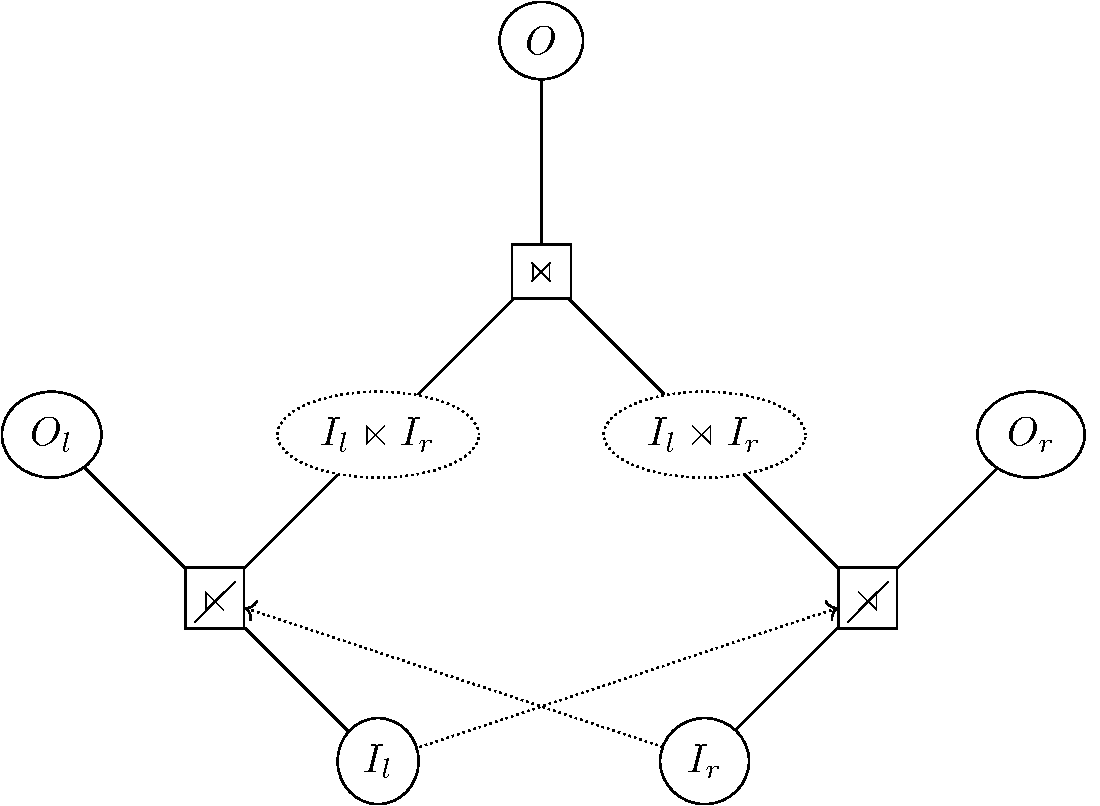
\includegraphics[width=.9\linewidth]{./imgs/example_metaop.pdf}
\caption{\label{fig:example_metaop}starting at n-node \(O\), the output
  of a join operation, we can derive three MetaOps that can
  materialize it.
  \(MetaOp\{in: \langle I_l, I_r \rangle, out: \langle O \rangle \}\),
  \(MetaOp\{in: \langle I_l, I_r \rangle, out: \langle O_l, O \rangle
  \}\),
  \(MetaOp\{in: \langle I_l, I_r \rangle, out: \langle O, O_r \rangle
  \}\),
  \(MetaOp\{in: \langle I_1, I_2 \rangle, out: \langle O_l, O, O_r
  \rangle \}\). Because trying all combinations of outputs explodes
  the search space we always go for the largest and then let the
  garbage collector deal with the possible repercussions. On the other
  hand to materialize \(I_l\) there is only one \hask{MetaOp} that
  relates to this cluster
  \(MetaOp\{in:\langle O, O_l \rangle, out: \langle I_l \rangle,
  interm: \langle I_l \lsemi I_r \rangle \}\)}
\end{figure}

\begin{code}
\begin{haskellcode}
data MetaOp t n = MetaOp {
  metaOpIn     :: NodeSet n,
  metaOpOut    :: NodeSet n,
  metaOpInterm :: NodeSet n,
  metaOpPlan   :: forall m' . Monad m' => PlanT t n m' [Transition t n]
  }
\end{haskellcode}
  \caption{\label{lst:metaop_def}A \hask{MetaOp} refers to input,
    output, and intermediate n-nodes that are involved in the set of
    operations it abstracts. Furthermore, it contains a computation
    that registers and returns the transitions involved in the
    \hask{MetaOp}.}
\end{code}


Two questions should arise from the above description: a) how does the
planner avoid cycles where it recursively tries to materialize the
parents and then the children? and b) how does it know not to
materialize an n-node twice? Both those problems are addressed by
refining the possible states of the n-nodes (listing
\ref{lst:ismat_def}). Rather than being just \hask{Mat} or
\hask{NoMat}. We also disambiguate between \hask{Initial} and
\hask{Concrete} n-nodes. N-nodes in the \hask{Initial} state are allowed
to change their materialization status. In contrast \hask{Concrete}
n-nodes have their state fixed with very few exceptions. Then, when an
n-node is asserted to be materialized, its status is first checked and
following scenaria are possible:

\begin{itemize}
\item The n-node's status found to be \hask{Concrete} and \hask{NoMat}
  and the branch immediately fails as it is not allowed to be set to
  materialized.
\item If it is \hask{Concrete} and \hask{Mat} the assertion simply
  succeeds
\item If it is \hask{Initial} and \hask{Mat} it is turned into
  \hask{Concrete} and \hask{Mat} and the assertion succeeds.
\item If the n-node's status is \hask{Initial} and also \hask{NoMat},
  two things need to happen: first, the n-ode is set \hask{Concrete} and
  \hask{NoMat} in order to avoid cycles, and the aforementioned
  process of finding a \hask{MetaOp} is carried out recursively in
  order to materialize the n-node.
\end{itemize}

\begin{code}
\begin{haskellcode}
data IsMat = Mat | NoMat
data NodeState =
  -- Concretified states are allowed to change only within the same
  -- lexical scope.
  Concrete IsMat
  -- Initial states are subject to change when encountered as a
  -- neighbour or by the GC.
  | Initial IsMat
\end{haskellcode}
  \caption{\label{lst:ismat_def}The different states that an n-node is
    allowed to be in.}
\end{code}

Once an n-node's is materialized and we start materializing its
siblings, it is important that the garbage collector (which we will be
discussing in section \ref{sec:gc}) does not delete the said n-node. To
avoid this, n-nodes materialized are set to \hask{Concrete Mat}
until all their siblings, that are inputs to the same \hask{MetaOp},
are materialized. Once the \hask{MetaOp} is triggered and its output
n-nodes are set to the \hask{Concrete Mat} state the input n-nodes are set
to \hask{Initial Mat} as it is now safe for the garbage collector to
remove them.

It is worth highlighting the importance of each n-node in a dependency set of an n-node
being \emph{completely} materialized before the process of materializing the
next one commences, i.e., that no two sibling n-nodes are
simultaneously in the process of being materialized. The reason is
that at any time a single trail of parent n-nodes is marked as
\hask{Concrete} and \hask{NoMat}, otherwise we cannot be sure whether a
\hask{Concrete NoMat} n-node that renders a \hask{MetaOp}
non-triggerable is actually in the process of becoming materialized,
meaning that when that process succeeds the \hask{MataOp} under
consideration will be triggerable.

\subsection{Garbage collection}
\label{sec:gc}

One of the fundamental design decisions of FluiDB is that she is
commited to materializing all intermediate n-nodes, a la MonetDB \cite{monetdb}, and keeping them
around for as long as possible. On the one hand, the plan selected is
crafted so that the intermediate query results are maximally useful for the
overall workload, on the other, when the available storage runs out,
the \emph{garbage collector} (GC) mechanism selects the least useful n-nodes to be
deleted, freeing the pages required for planning the query. In this section
we focus on the latter.

The garbage collector is triggered right before a \hask{MetaOp} is to
be triggered. It calculates the space required for materializing the
output n-nodes and the space available to decide whether inserting a
plan fragment generated by a GC run is required. Then it selects a
subset of materialized n-nodes to delete in order to make room for the
new results and inserts \hask{DelNode <n-node>} transitions for each one into the
plan. The selection process has two hard constraints:

\begin{itemize}
\item The n-nodes being deleted must be \emph{deletable}, i.e. the
  n-node's state is \hask{Initial} and if the n-node is deleted that it
  can be reconstructed from the remaining materialized n-nodes. 
  \footnote{There is a caveat to our conception of deletability of nodes, namely that 
  the concept does not take into account budgetary constraints, only that there is no 
  loss of information resulting from the relation's deletion.}
\item The n-nodes being deleted must not be required for the
  continuation of the current plan. We call these n-nodes
  \emph{protected}. For example, say we are planning for the query
  \(A \Join B\) and we have materialized \(A\) already but while
  materializing \(B\) the GC is triggered. \(A\) should not be in the
  repertoire of n-nodes the GC can delete under any circumstances.
\end{itemize}

Selecting a subset of n-nodes for deletion is not an easy problem, so we follow a
simple heuristic (see listing \ref{lst:gc_algo}). 
Large n-nodes are costly to create and therefore the larger the n-node,
the less inclined the planner is to create it, and the more useful it
is likely to be. With that in mind, the heuristic we follow is for the
garbage collector to prioritise deleting small n-nodes over deleting
larger ones.

The first order of business for the GC the is to find the set of
deletable n-nodes and sort them by size. It tries to delete them one by
one starting from the smaller ones and working its way up to the
larger ones. Every time a n-node is deleted, it is possible that other
n-nodes that were previously established to be deletable lose that
property. For example, if n-nodes \(A\), \(\sigma_p A\), and
\(\sigma_{\neg p} A\) are \hask{Initial} and materialized and not
connected to other n-nodes but to each other, each one of
them can be materialized from the others and therefore all of them are
marked as deletable. If the GC deletes \(A\) first, the other
two are no longer deletable as neither would be materializable were they
to be deleted.

N-nodes that are established as non-deletable in this way are switched
from \hask{Initial} to \hask{Concrete} to avoid re-calculating their
materializability.

If after this process not enough space is created, the GC resorts to
starting a new \emph{planner epoch}. The function of a planner epoch
change is for the planner to revisit the assumptions that it has made in
the form of setting n-nodes to \hask{Concrete Mat}. That is to say, when a new
epoch begins, the unprotected n-nodes materialized in the current run
become available for deletion and all the
n-nodes states and transitions that were recorded since the last planner
epoch started are stashed into the epoch stack. The epoch stack
resides in the branch-local state (\hask{GCState}) and contains a map
of n-nodes to their states at the end of the epoch and a sequence of
transitions. When a new epoch is pushed into the stack, a new mapping
of states is created according to the following rules:

\begin{itemize}
\item The materialization status (\hask{Mat} or \hask{NoMat}) does not change between epochs: All
  materialized n-nodes from the previous epoch are materialized in the
  new one materialized and all non-materialized n-nodes are still not
  materialized.
\item All non-protected \hask{Concrete} n-nodes become \hask{Initial}
  n-nodes.
\end{itemize}

The sequence of transitions for the new epoch is empty. The reason we
keep separate lists of transitions is, as we will see in more detail
in the code generation chapter, that the subset of output n-nodes that a
physical operation generates is established at the time of physical
planning based on the materialized n-nodes according to the epoch
corresponding to the transition.

An epoch contains important information about the state of the
planner. For this reason, when an epoch is inserted in the stack it is
checked for equality against the other epochs in the stack. If two
equivalent epochs are inserted in the stack the branch fails
permanently as it means that there is a cycle.

This enables another optimization, the \emph{free-to-delete} n-nodes. As
mentioned previously, the planner prioritizes the version of
\hask{MetaOps} that materializes all outputs for example it will
prioritize the branch that follows
\(MetaOp\{in=\langle A \rangle, out=\langle \sigma_p A, \sigma_{\neg
  p} A \rangle \}\) over the one that follows
\(MetaOp\{in=\langle A \rangle, out=\langle \sigma_p A \rangle
\}\). It is rarely the case, however, that all the outputs are
required. In this example,
triggering the former \hask{MetaOp} and then garbage collecting
\(\sigma_{\neg p} A\) without it being used is never desirable. For
that reason we mark the n-node \(\sigma_{\neg p} A\) as
\emph{free-to-delete} as soon as it is created based on the fact that
it is not required. When the garbage collector deletes free-to-delete
n-nodes it does so without registering a deletion transition. This way
the physical planner will generate a plan where \(\sigma_{\neg p} A\)
is never created in the first place. All n-nodes lose their
free-to-delete status upon the creation of a new epoch.

\begin{code}
\begin{haskellcode}
gc reqSize = do
  -- Try the current epoch and if that fails retry with a new epoch.
  return () <//> newEpoch
  -- find the deletable n-nodes and sort them by size
  deleteables <- sortOnM getNodeSize =<< filterM isDeletable =<< getAllNodes
  -- Try deleting each n-node and stop deleting when amassing enough
  -- free pages.
  forM_ deletables $ \n -> do
    freePgs <- getFreePages
    when (freePgs < reqSize) $ tryDelete n <//> markAsConcrete n


-- | Try to delete an n-node.
tryDelete node = do
  -- check that the n-node is still deletable
  guardM $ isDeletable node
  -- If it is free-to-delete do not register the DelNode trigger
  isFreeToDel <- getIsFreeToDel node
  unless isFreeToDel $ register $ DelNode node
  -- Mark the n-node as not materialized.
  setStatus node (Initial NoMat)


-- | Check that an n-node is deletable
isDeletable n = do
  st <- getNodeState n
  case st of
    Initial Mat -> do
      -- Only nodes in Initial Mat state might be deletable. Try deleting
      -- and check that it is materializable.
      setNodeState n (Initial NoMat)
      ret <- isMaterializable n
      setNodeState n (Initial Mat)
      return ret
    _ -> return False

-- | An n-node that was not deletable should not be considered again
-- for deletion and is therefore marked as concrete.
markAsConcret n = do
  st <- getNodeState n
  case st of
    Initial m -> setNodeState (Concrete m)
    _ -> return ()
\end{haskellcode}
  \caption{\label{lst:gc_algo}A sketch of the garbage collector
    algorithm in pseudo-haskell.}
\end{code}

It is hopefully clear at this point that the process of garbage
collection involves a large search space. We sacrifice some of our
plan repertoire by running the entire process wrapped in a \hask{once}
operator that we described in the previous section.

Finally, a word about protected n-nodes. N-nodes are protected within the
context of a branch from the time they are established as part of the
input set of a \hask{MetaOp} we are making triggerable until the time said
\hask{MetaOp} is actually triggered during the normal planning (i.e. not
the GC). Because an n-node may be the input of more than one
simultaneously considered \hask{MetaOps}, protection of a n-node is not a
boolean value that is set when the n-node is encountered as \hask{MetaOp}
input and unset when the \hask{MetaOp} is triggered, but rather an natural
number variable that is incremented and decremented respectively. When
that value is zero, the n-node is not considered protected.


\subsection{Order of traversal}

We mentioned that the \hask{MetaOps} are selected
non-deterministically. In this section, we will go in depth on the
FluiDB planner's strategy on the order in which it considers its
options using the \hask{HCntT} framework, making heavy use of the
\hask{halt} operator to decide branch priorities. A branch's priority
is dependent on the particular frontier at the time of a halt and is
determined by four factors:

\begin{itemize}
\item The cost of the \hask{MetaOp}s that the branch is in the process
  of making triggerable.
\item The cost of the \hask{MetaOp}s that have \emph{already been triggered}.
\item The sum of the estimated costs of \emph{each n-node in the frontier}.
\item A weighted sum of the \emph{stochastic cost} of historical queries based
on the current frontier.
\end{itemize}

The final two factors are values on which we will focus in this
section. They are computed often and are dependent on the set of
materialized n-nodes. Since the set of materialized n-nodes does not
change in a completely arbitrary way from computation to computation a
naive approach to calculating those values would involve a lot of
duplicate work. For this reason, we use Antisthenis which will be
expanded in a chapter \ref{chapter:antisthenis} to minimize the amount
of work required.

We define a very rough way
of estimating cost materializing n-nodes. We incrementally estimate the cost of each n-node
of the frontier using the following formula:

\begin{align*}
  c_{nomat}(n) &=
    \min\limits_{op \in \text{metaops with \(n\) output}} \left\{ cost(op) + \sum\limits_{i \in inputs(op)} c(i)  \right\} \\
  c_{mat}(n) &= 0
\end{align*}

Where the cost \(c(n)\) of n-node \(n\) is \(c_{mat}(n)\) if the n-node
is materialized and \(c_{nomat}(n)\) otherwise. In plain english the
cost is recursively estimated as the cheapest combination \hask{MataOp}
plus the cost of materializing the input n-nodes.

This approach has several problems like the fact that n-nodes that are
used more than once are also added more than once and that it does not take
at all into account the budget constraints. It is, however, a good
enough heuristic for prioritizing branches.

The final factor, which takes into account the historical queries is a
bit more tricky. The planner keeps track of the last couple of queries
requested and the corresponding n-nodes, and tries to estimate how
beneficial following the current branch would be in the event where
a query similar to those is requested in the future. We estimate that
by summing up a slightly different notion of cost for those queries.

A naive approach would be to just use the the same algorithm as we did
for the frontier n-nodes. However, this approach is prone to getting
stuck behind materialized n-nodes: past queries, especially recent ones,
are likely to still be materialized and therefore their cost is likely
to be 0. Even if the GC has already got around to deleting them, their near
dependencies are likely to be materialized and block the cost estimator 
from traversing the graph up to the nodes affected by the current plan. This makes
the estimation quite bad for two reasons:

\begin{itemize}
\item N-nodes found to be materialized when prioritizing branches may have been
  deleted by a GC pass by the time they are actually requested.
\item We do not care about the cost of the particular n-nodes, but rather
  about \emph{similar} n-nodes. For that reason we want to avoid
  depending too heavily on a particular materialized n-node being
  materialized.
\end{itemize}

A slightly better way of calculating the expected cost that an n-node will
have at a future point in time, which we
heuristically attempt to approximate, would be, instead of
considering the cost of materialized n-nodes to be zero, to calculate
the likelihood that a materialized n-node will still be materialized
when we encounter it again. This is related not only to an estimation
of how many page writes separate the moment of cost estimation and the
actual plan the cost of which is being estimated, but also all the
decisions that the garbage collector will make in that time. After
FluiDB's budget is exhausted for the first time, for every page write
a page needs to be garbage collected. We considered a couple of
options for stochastically modelling the behavior of the GC like
assuming that it chooses random pages or random tables to delete, but
we could find none that was both a mathematically justifiable approximation and
computationally viable.

For this reason, we decided to follow a pragmatic approach to the
problem and simply assume that for every materialized n-node there is a
constant probability that it will not still be materialized when we
need it, scaling the cost \(c_{nomat}\) of that n-node by that factor
to get the stochastic cost. Thus the cost formula \(h\) for the n-nodes
now is:

\begin{align*}
  h_{nomat}(n) &= \min\limits_{op \in \text{metaops with \(n\) output}} \left\{ h(op) + \sum\limits_{i \in inputs(op)} cost(i)  \right\} \\
  h_{mat}(n) &= \lambda \cdot h_{nomat}(n)
\end{align*}

Where \(\lambda \in [0,1]\) is the estimated probability that the
n-node is no longer materialized when needed. As before, materialized
n-nodes have cost \(c_{mat}\) and non-materialized n-nodes have cos
\(c_{nomat}\)

\section{Conclusion}

In this chapter we saw two distinct concepts: a weighted backtracking
framework and a system implemented on top of that framework, namely
the FluiDB's physical planner. These two combined enable FluiDB to
search for quality plans within the QDAG in a flexible way.
